\documentclass[12pt]{article}
\usepackage{amsmath}
\usepackage{array}
\usepackage{geometry}
\usepackage{graphicx}
\usepackage{hyperref}
\usepackage[latin1]{inputenc}
\usepackage{listings}
\usepackage{mathtools}
\renewcommand{\labelitemi}{$\textendash$}
\geometry{
    a4paper,
    total={170mm,257mm},
    left=15mm,
    right=15mm,
    top=5mm,
    bottom=15mm
}
\DeclarePairedDelimiter\floor{\lfloor}{\rfloor}

\title{CS4061: Week 8 Assignment}
\author{Conor McCauley - 17323203}
\date{December 1, 2020}

\begin{document}

\maketitle

\section*{Question (i)}

\noindent (a) The code from appendix A reads in an image and outputs two resulting images - one for each kernel. Inside of the convolution function the input array is first padded with zeros to ensure our resulting image is the same size as the input image - this is done with the following code:

\begin{center}
    \lstset{basicstyle=\footnotesize}
    \begin{lstlisting}[language=Python]
    pad = len(kernel) // 2
    array = np.pad(array, pad, mode='constant')
    \end{lstlisting}
\end{center}

For each pixel $(x, y)$ in our input array the formula used to calculate the corresponding result pixel is as follows:

$$result(x, y) = \sum_{kx = 0}^K \sum_{ky = 0}^K input(x + kx - \floor{\frac{K}{2}}, y + ky - \floor{\frac{K}{2}}) \cdot kernel(kx, ky)$$

\textbf{N.B.} the subtraction of $\floor{\frac{K}{2}}$ from $kx$ and $ky$ is done so that $kx = 0$ becomes -1, $kx = 1$ becomes 0, etc.

The above formula is implemented with the following code which is run for each $(x, y)$ in the input:

\begin{center}
    \lstset{basicstyle=\footnotesize}
    \begin{lstlisting}[language=Python]
    value = 0
    for kx in range(K):
        for ky in range(K):
            # offset kernel element
            ox = kx - (K // 2)
            oy = ky - (K // 2)
            # add to sum
            value += kernel[ky][kx] * array[y + oy][x + ox]
    result[y][x] = value
    \end{lstlisting}
\end{center}

\textbf{N.B.} the range of $(x, y)$ values that are considered depend on the size of the padded array, i.e., if the padded array is $N \cdot N$ and the size of the padding is $p$ then we will consider values in the range $p \le x, y < N - p$.

\noindent (b) The following image of a reddish pentagon was used as input:

\begin{center}
    
\includegraphics[scale=0.8]{part i/image.png}
\end{center}

The convolution is carried out on the image's red colour channel:

\begin{center}
    \lstset{basicstyle=\footnotesize}
    \begin{lstlisting}[language=Python]
    rgb = np.array(Image.open('image.png').convert('RGB'))
    red = rgb[:,:,0]
    result = convolve(red, kernel)
    \end{lstlisting}
\end{center}

The following images were produced by the \texttt{convolve()} function for the given kernels:

\begin{center}
    \begin{tabular}{>{\centering\arraybackslash}m{3.5cm}>{\centering\arraybackslash}m{3.5cm}}
         Kernel & Image \\
         \hline \\
         $\begin{bmatrix} -1 & -1 & -1 \\ -1 & 8 & -1 \\ -1 & -1 & -1 \end{bmatrix}$ & 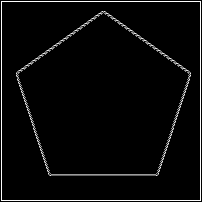
\includegraphics[scale=0.5]{part i/result1.png} \\
         $\begin{bmatrix} 0 & -1 & 0 \\ -1 & 5 & -1 \\ 0 & -1 & 0 \end{bmatrix}$ & 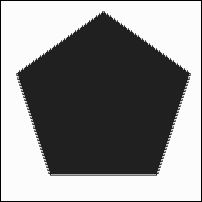
\includegraphics[scale=0.5]{part i/result2.png} \\
    \end{tabular}
\end{center}

The first kernel appears to perform some kind of edge detection on the input image based on the fact that only the outline of the pentagon is visible. The second kernel appears to perform a kind of sharpening since the outline of the pentagon becomes a lot more jagged in the resulting image.

\section*{Question (i)}

\noindent (a) The convolutional network (CN) uses 32x32 RGB images as input data meaning each input contains three channels - our input shape is therefore (32, 32, 3). The CN consists of four layers with each layer using a 3x3 kernel and `same' padding (meaning the input is padded with zeros to ensure the output is the same size as the input). The first two layers each contain 16 filters while the third and fourth layers each contain 32 filters - this means that the first two layers will contain 16 output channels while the third and fourth layers will contain 32 output channels. The second and fourth layers use a 2x2 stride, leading to smaller output matrices (downsampling). The first and third layers use a 1x1 stride, leading to output matrices which are the same size as the input. Each of these layers use a ReLU activation function. The CN also contains a dropout layer to reduce the risk of overfitting, a flattening layer to convert output tensors into vertices and a dense layer (or fully-connected layer) which uses a softmax activation function.

\noindent (b)

\indent (i) Keras reports that this model has $37146$ parameters in total. The layer with the most parameters leading into it is the final \texttt{Dense} layer with $20490$ parameters. The reason for this is as follows: our final convolution layer has an output shape of $(8, 8, 32)$ which results in $8 \cdot8 \cdot 32 = 2048$ parameters - this output is then passed through the \texttt{Dropout} and \texttt{Flatten} layers (while retaining the same number of parameters) before being handled by the final \texttt{Dense} layer. The final layer will consist of $10$ outputs (one for each class) and, in order to `fully connect' our $2048$ previous parameters with our $10$ outputs, we will need $2048 \cdot 10 = 20480$ parameters. However, each of the outputs also has a bias parameter which results in $20490$ parameters in total.

The model reported an accuracy of $50\%$ on the test data and an accuracy of $63\%$ on the training data. This decrease in performance when predicting against test data is to be expected due to the fact that the data is entirely new and unseen. For comparison, a simple baseline that always predicted the most common label, which in my case was the 9th label, would report an accuracy of $10.4\%$ on the training data and $10\%$ on the test data. It is clear that our trained model, even though it only achieves an accuracy of $50\%$ against test data, is far superior to our baseline model.

\indent (ii) The code produced the following plot:

\begin{center}
    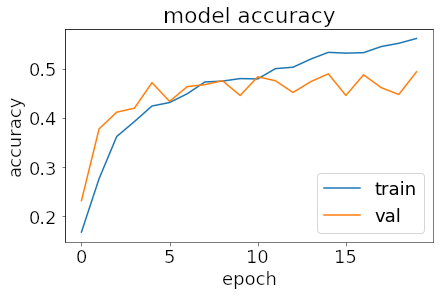
\includegraphics[scale=0.6]{part ii/fig_1.png}
\end{center}

For the first two or three epochs neither the training data nor the validation data provide very accurate results and it is clear that our model is under-fitting to some degree. Over the next few epochs, although the accuracy of both datasets are relatively high, the validation predictions are actually more accurate than the training predictions - this is also an indication that our model is still under-fitting. In the final few epochs the training data begins to outperform the validation data by a relatively large margin. This could be an indication that our model is beginning to over-fit due to it not generalising to the validation data very well.

\indent (iii) We can measure the length of time taken to train our model with the following code:

\begin{center}
    \lstset{basicstyle=\footnotesize}
    \begin{lstlisting}[language=Python]
    start_time = time.time()
    model.fit(...)
    end_time = time.time()
    print(f'Time taken: {end_time - start_time} seconds')
    \end{lstlisting}
\end{center}

The raw results from running the convolutional network for different sized training sets are summarised in the following table:

\begin{center}
    \begin{tabular}{|c|c|c|c|c|}
        \hline
        Training points & Time taken & Training accuracy & Test accuracy \\ \hline
        5K & 90s & 63\% & 50\% \\
        10K & 180s & 68\% & 58\% \\
        20K & 375s & 70\% & 62\% \\
        40K & 756s & 73\% & 68\% \\
        \hline
    \end{tabular}
\end{center}

From the running times listed in the above table it would seem that doubling the number of points in the training data leads to a running time that is twice as long as the previous time. This would suggest that there is a linear relationship between the size of the dataset and the time taken to train the model.

\textbf{N.B.} for each trained model the baseline accuracy remained roughly the same: 10\%.

In every case an increase in the number of training points led to an increase in both the accuracy of the model with training data and the accuracy of the model with test data. The increase in accuracy seen with the test data was always higher than the increase in accuracy with the training data. It seems that doubling the size of the dataset will lead to a similar doubling in the time taken to train the model while only resulting in a small increase in the model's predictive accuracy. Nonetheless, out of the above dataset sizes it would seem that 40K training points is still the most suitable choice as, relatively speaking, it doesn't take too long to run while achieving a test accuracy of almost 68\% - a 18\% increase over the dataset with 5K points.

The following plots display the history variable for each trained model:

\begin{center}
    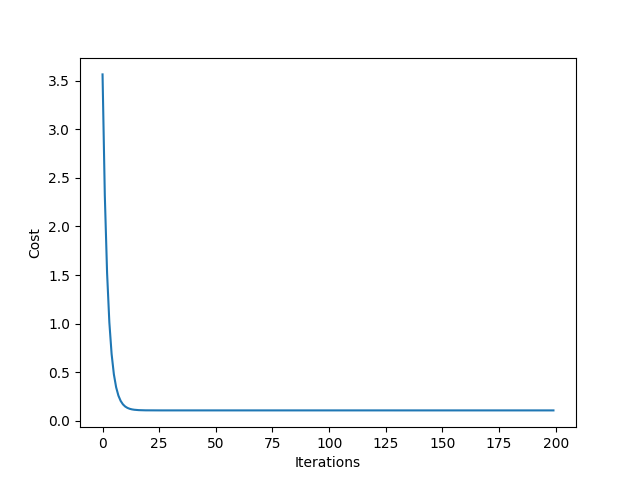
\includegraphics[scale=2.0]{part ii/fig_2.png}
\end{center}

In each instance for the first few epochs the model is under-fitting for both the training data and the validation data. Over the next few epochs, as discussed in (ii), the accuracy of each of the models begin to steadily increase while the validation data remains slightly more accurate. In the final few epochs, however, only the 5K model begins to see a large divergence between the accuracy of the training data and the accuracy of the validation data. Both the 10K and 20K models only show a small increase in accuracy over the validation data while the 40K model never actually sees the training data outperforming the validation data. It seems that, in this case, the larger our training dataset is the closer the validation accuracy and training accuracy become which indicates that our model is neither under-fitting or over-fitting the dataset. These later results further imply that the 40K model might be the optimal choice here.

\indent (iv) I chose to use the following wide range of parameter values:

$$L_1 \in \{ 0, 0.00001, 0.0001, 0.001, 0.01, 0.1, 1 \}$$.

Training the model with these weight parameters results in the following reported accuracies:

\begin{center}
    \begin{tabular}{|c|c|c|}
        \hline
        $L_1$ & Training accuracy & Test accuracy \\ \hline
        0 & 61\% & 51\% \\
        0.00001 & 63\% & 49\% \\
        0.0001 & 64\% & 51\% \\
        0.001 & 63\% & 50\% \\
        0.01 & 44\% & 42\% \\
        0.1 & 37\% & 36\% \\
        1 & 10\% & 10\% \\
        \hline
    \end{tabular}
\end{center}

From this table we can see that for values of $L_1 > 0.001$ there is a sharp decline in both training and test accuracy. In fact, a value of $L_1 = 1$ results in an accuracy no better than our baseline. For the values of $L_1 \le 0.001$ we see that both the training and test accuracies remain fairly consistent (with the exception of $L_1 = 0$ which has a slightly lower training accuracy). Given these results it would appear that values of $L_1 \in \{ 0.00001, 0.0001, 0.001 \}$ would all be perfectly acceptable choices - with $L_1 = 0.0001$ being slightly better than the rest in both training and test accuracy.

\noindent (c)

\indent (i) In order to implement max-pooling we only need to change a few lines of code - we can simply define our model using the following code:

\begin{center}
    \lstset{basicstyle=\footnotesize}
    \begin{lstlisting}[language=Python]
    model = keras.Sequential()
    model.add(Conv2D(16, (3,3), padding='same', input_shape=x_train.shape[1:],
        activation='relu'))
    model.add(Conv2D(32, (3,3), padding='same', activation='relu'))
    model.add(MaxPooling2D(pool_size=(2, 2), padding="same"))
    model.add(Dropout(0.5))
    model.add(Flatten())
    model.add(Dense(num_classes, activation='softmax',
        kernel_regularizer=regularizers.l1(0.001)))
    \end{lstlisting}
\end{center}

This will create a 16 channel `same' layer, a 32 channel `same' layer and a max-pool layer with a size of (2, 2). We can retain the dropout, flatten and dense layers from our previous model.

\indent (ii) Keras reports that this model has 87018 parameters in total with the final dense layer having 81930 parameters. This large increase in parameters over our previous model is to be expected since our 32 channel layer has an output shape of $(16, 16, 32)$ which results in a total of 8192 parameters - each of these parameters much be connected to each of the 10 outputs of the dense layer (which also includes 10 bias parameters) leading to $8192 \cdot 10 + 10 = 81930$ parameters for the dense layer alone.

It took 163 seconds to train this model on 5K points - nearly twice the amount of time taken to train our previous model on 5K points (90 seconds). This increase in running time is most likely due to the large increase in the number of parameters the model has due to the fact that the values of each of these parameters must be repeatedly updated and evaluated while training the model.

This model reports training and test accuracies of 58\% and 48\%, respectively. These results are a bit worse than our previous model's reported accuracies of 63\% and 50\%. This poorer performance, as well as the longer running time, would indicate that this exact max-pool model design is a worse choice than our previous model.

\section*{Appendix A: Code for (i)}

\lstset{basicstyle=\footnotesize}
\begin{lstlisting}[language=Python]
import numpy as np
from PIL import Image

def convolve(array, kernel):
    # pad the input array with zeros
    pad = len(kernel) // 2
    array = np.pad(array, pad, mode='constant')
    
    # get array and kernel dimensions
    N = len(array)
    K = len(kernel)
    
    # init result array
    result = np.zeros((N, N))
    
    # for each pixel in the image (ignoring the padding)
    for x in range(pad, N - pad):
        for y in range(pad, N - pad):
            value = 0
            # for each element in the kernel
            for kx in range(K):
                for ky in range(K):
                    # offset kernel element
                    ox = kx - (K // 2)
                    oy = ky - (K // 2)
                    # add to sum
                    value += kernel[ky][kx] * array[y + oy][x + ox]
            result[y][x] = value
    
    return result

def main():
    rgb = np.array(Image.open('image.png').convert('RGB'))
    red = rgb[:,:,0]
    kernel1 = np.array([[-1,-1,-1],[-1,8,-1],[-1,-1,-1]])
    kernel2 = np.array([[0,-1,0],[-1,8,-1],[0,-1,0]])
    result1 = convolve(red, kernel1)
    result2 = convolve(red, kernel2)
    image1 = Image.fromarray(np.uint8(result1))
    image2 = Image.fromarray(np.uint8(result2))
    image1.show()
    image2.show()
    image1.save('result1.png')
    image2.save('result2.png')

main()
\end{lstlisting}

\section*{Appendix B: Code for (ii)}

\lstset{basicstyle=\footnotesize}
\begin{lstlisting}[language=Python]
import numpy as np
import tensorflow as tf
from tensorflow import keras
from tensorflow.keras import layers, regularizers
from keras.layers import Dense, Dropout, Activation, Flatten, BatchNormalization
from keras.layers import Conv2D, MaxPooling2D, LeakyReLU
from sklearn.metrics import confusion_matrix, classification_report
from sklearn.utils import shuffle
import matplotlib.pyplot as plt
plt.rc('font', size=18)
plt.rcParams['figure.constrained_layout.use'] = True
import sys
import time

# Model / data parameters
num_classes = 10
input_shape = (32, 32, 3)

# the data, split between train and test sets
(x_train, y_train), (x_test, y_test) = keras.datasets.cifar10.load_data()
n=5000#5000,10000,20000,40000
x_train = x_train[1:n]; y_train=y_train[1:n]
#x_test=x_test[1:500]; y_test=y_test[1:500]

# Scale images to the [0, 1] range
x_train = x_train.astype("float32") / 255
x_test = x_test.astype("float32") / 255
print("orig x_train shape:", x_train.shape)

# convert class vectors to binary class matrices
y_train = keras.utils.to_categorical(y_train, num_classes)
y_test = keras.utils.to_categorical(y_test, num_classes)

# calculate occurences of labels in data (for baseline)
labels_train = [0] * num_classes
for yt in y_train:
	ixs = np.where(yt == 1)
	labels_train[ixs[0][0]] += 1
labels_test = [0] * num_classes
for yt in y_test:
	ixs = np.where(yt == 1)
	labels_test[ixs[0][0]] += 1
print(labels_train)
print(labels_test)

is_part_c = False # if is_part_c then use max pooling, etc
use_saved_model = False
if use_saved_model:
	model = keras.models.load_model("cifar.model")
else:
	model = keras.Sequential()
	if is_part_c:
		model.add(Conv2D(16, (3,3), padding='same', input_shape=x_train.shape[1:],
		    activation='relu'))
		model.add(Conv2D(32, (3,3), padding='same', activation='relu'))
		model.add(MaxPooling2D(pool_size=(2, 2), padding="same"))
	else:
		model.add(Conv2D(16, (3,3), padding='same', input_shape=x_train.shape[1:],
		    activation='relu'))
		model.add(Conv2D(16, (3,3), strides=(2,2), padding='same',
		    activation='relu'))
		model.add(Conv2D(32, (3,3), padding='same', activation='relu'))
		model.add(Conv2D(32, (3,3), strides=(2,2), padding='same',
		    activation='relu'))
	model.add(Dropout(0.5))
	model.add(Flatten())
	l1_param = 0.001#0,0.00001,0.0001,0.001,0.01,0.1,1
	model.add(Dense(num_classes, activation='softmax',
	    kernel_regularizer=regularizers.l1(l1_param)))
	model.compile(loss="categorical_crossentropy", optimizer='adam',
	    metrics=["accuracy"])
	model.summary()

	batch_size = 128
	epochs = 20
	start_time = time.time()
	history = model.fit(x_train, y_train, batch_size=batch_size, epochs=epochs,
	    validation_split=0.1)
	end_time = time.time()
	print('==========================')
	print(f'Time taken: {end_time - start_time} seconds')
	print('==========================')
	model.save("cifar.model")
	#plt.subplot(211)
	plt.plot(history.history['accuracy'])
	plt.plot(history.history['val_accuracy'])
	plt.title('model accuracy')
	plt.ylabel('accuracy')
	plt.xlabel('epoch')
	plt.legend(['train', 'val'], loc='lower right')
	"""plt.subplot(212)
	plt.plot(history.history['loss'])
	plt.plot(history.history['val_loss'])
	plt.title('model loss')
	plt.ylabel('loss'); plt.xlabel('epoch')
	plt.legend(['train', 'val'], loc='lower right')"""
	plt.show()

preds = model.predict(x_train)
y_pred = np.argmax(preds, axis=1)
y_train1 = np.argmax(y_train, axis=1)
print(classification_report(y_train1, y_pred))
print(confusion_matrix(y_train1,y_pred))

preds = model.predict(x_test)
y_pred = np.argmax(preds, axis=1)
y_test1 = np.argmax(y_test, axis=1)
print(classification_report(y_test1, y_pred))
print(confusion_matrix(y_test1,y_pred))
\end{lstlisting}

\end{document}
